\chapter{Implementasi dan Pengujian}
\label{chap:implementasipengujian}

Bab ini membahas tentang implementasi dan pengujian perangkat lunak berdasarkan rancangan yang sudah dibuat. Ada dua jenis pengujian yang dilakukan, yaitu pengujian fungsional, dan pengujian eksperimental. Bab ini juga membahas tentang lingkungan yang digunakan untuk pengujian perangkat lunak ini.

\section{Lingkungan untuk Pengujian}
\label{sec:lingkunganpengujian}

Ada dua jenis lingkungan untuk pengujian perangkat lunak ini, yaitu:

\begin{enumerate}
\item Lingkungan perangkat keras
\item Lingkungan perangkat lunak
\end{enumerate}

Pengujian perangkat lunak ini dilakukan di Lab Komputasi FTIS Unpar ruang 9018. Kedua jenis lingkungan tersebut akan dibahas lebih lanjut dibawah ini.

\subsection{Lingkungan Perangkat Keras}
\label{sec:lingkunganpk}

Lingkungan perangkat keras yang digunakan untuk pengujian perangkat lunak ini memiliki spesifikasi berikut:

\begin{table}
\centering
\captionsetup{justification=centering}
\caption[Lingkungan perangkat keras untuk pengujian perangkat lunak]{Lingkungan perangkat keras untuk pengujian perangkat lunak}
\begin{tabular}{| l | l |}
\hline
Parameter & Nilai \\
\hline \hline
\textit{Processor} & Lorem Ipsum \\
\hline
\textit{RAM (Random Access Memory)} & Lorem Ipsum \\
\hline
\textit{VGA (Video Graphics Array)} & Lorem Ipsum \\
\hline
\end{tabular}
\label{tab:lingkunganpk}
\end{table}

\subsection{Lingkungan Perangkat Lunak}
\label{sec:lingkunganpl}

Lingkungan perangkat perangkat lunak yang digunakan untuk pengujian perangkat lunak ini memiliki spesifikasi berikut:

\begin{table}
\centering
\captionsetup{justification=centering}
\caption[Lingkungan perangkat lunak untuk pengujian perangkat lunak]{Lingkungan perangkat lunak untuk pengujian perangkat lunak}
\begin{tabular}{| l | l |}
\hline
Parameter & Nilai \\
\hline \hline
Sistem Operasi & Lorem Ipsum \\
\hline
Bahasa Pemrograman & Java \\
\hline
\textit{IDE (Integrated Development Environment)} & NetBeans IDE 8.2 \\
\hline
\textit{Library Java} & JDK (\textit{Java Development Kit}) 1.8 \\
\hline
\textit{JVM (Java Virtual Machine)} & Java Version 8 Update Lorem Ipsum \\
\hline
\end{tabular}
\label{tab:lingkunganpl}
\end{table}

\section{Implementasi}
\label{sec:implementasi}

Hasil implementasi dari rancangan perangkat lunak yang sudah dibuat ini terdiri dari dua bagian, yaitu:

\begin{enumerate}
\item Kode program
\item Antarmuka perangkat lunak
\end{enumerate}

Kedua bagian tersebut akan dibahas lebih lanjut di bawah ini.

\subsection{Kode Program}
\label{sec:kodeprogram}

Kode program untuk perangkat lunak ini ditulis dalam bahasa pemrograman Java, berdasarkan dengan rancangan diagram kelas yang sudah dibuat, seperti dapat dilihat pada sub-bab~\ref{sec:diagramkelas}. Seluruh kode program untuk perangkat lunak ini dapat dilihat di bab Lampiran.

\subsection{Antarmuka Perangkat Lunak}
\label{sec:antarmukapl}

Antarmuka untuk perangkat lunak ini dirancang berdasarkan rancangan yang sudah dibuat, seperti dapat dilihat pada sub-bab~\ref{sec:perancanganantarmuka}. Gambar~\ref{fig:antarmukapl1} menunjukkan antarmuka perangkat lunak saat pertama kali dibuka, sebelum \textit{file} permainan dibuka. Gambar~\ref{fig:antarmukapl2} menunjukkan kotak dialog untuk memilih \textit{file} permainan yang akan dibuka. Gambar~\ref{fig:antarmukapl3} menunjukkan antarmuka perangkat lunak setelah membuka \textit{file} permainan yang dipilih. Gambar~\ref{fig:antarmukapl4} menunjukkan kotak dialog untuk mengatur nilai untuk parameter-parameter algoritma genetik. Gambar~\ref{fig:antarmukapl5} menunjukkan antarmuka perangkat lunak setelah permainan berdasarkan \textit{file} permainan yang telah dibuka diselesaikan.

\begin{figure}
\centering
\captionsetup{justification=centering}
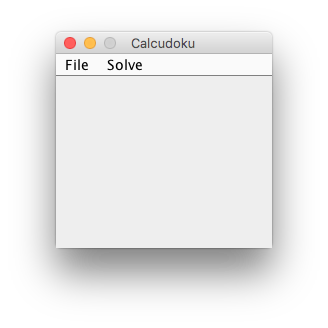
\includegraphics[scale=1]{Gambar/ImplementasiPengujian/Calcudoku1.png}
\caption[Antarmuka perangkat lunak saat pertama kali dibuka]{Antarmuka perangkat lunak saat pertama kali dibuka}
\label{fig:antarmukapl1}
\end{figure}

\begin{figure}
\centering
\captionsetup{justification=centering}
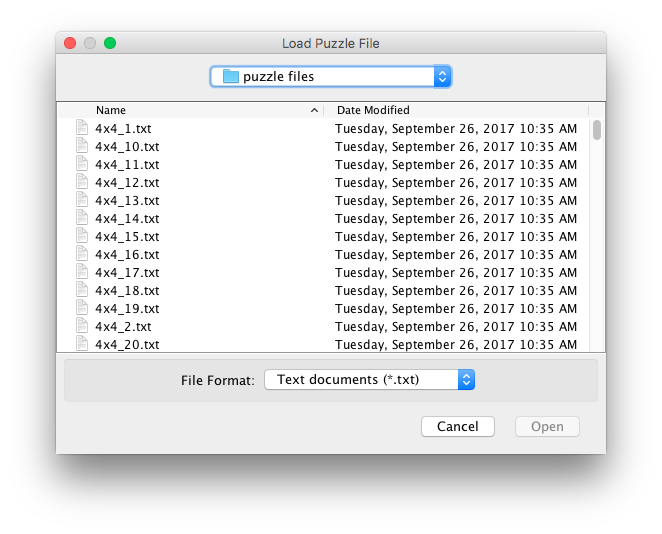
\includegraphics[scale=0.5]{Gambar/ImplementasiPengujian/FileChooser.png}
\caption[Kotak dialog untuk memilih \textit{file} permainan yang akan dibuka]{Kotak dialog untuk memilih \textit{file} permainan yang akan dibuka}
\label{fig:antarmukapl2}
\end{figure}

\begin{figure}
\centering
\captionsetup{justification=centering}
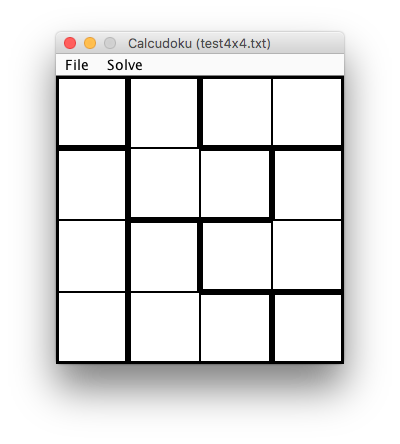
\includegraphics[scale=0.5]{Gambar/ImplementasiPengujian/Calcudoku2.png}
\caption[Antarmuka perangkat lunak sesudah membuka \textit{file} permainan yang dipilih]{Antarmuka perangkat lunak sesudah membuka \textit{file} permainan yang dipilih}
\label{fig:antarmukapl3}
\end{figure}

\begin{figure}
\centering
\captionsetup{justification=centering}
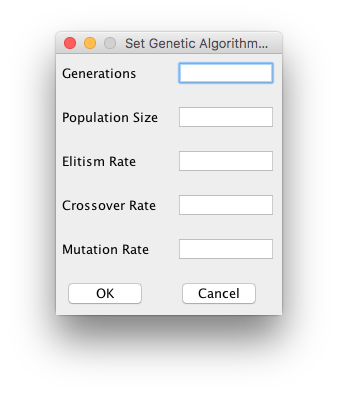
\includegraphics[scale=0.5]{Gambar/ImplementasiPengujian/SetGAParameters.png}
\caption[Kotak dialog untuk mengatur nilai dari parameter-parameter algoritma genetik]{Kotak dialog untuk mengatur nilai dari parameter-parameter algoritma genetik}
\label{fig:antarmukapl4}
\end{figure}

\begin{figure}
\centering
\captionsetup{justification=centering}
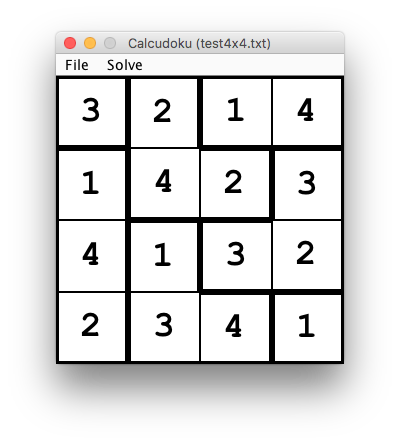
\includegraphics[scale=0.5]{Gambar/ImplementasiPengujian/Calcudoku3.png}
\caption[Antarmuka perangkat lunak setelah permainan berdasarkan \textit{file} permainan yang telah dibuka diselesaikan]{Antarmuka perangkat lunak setelah permainan berdasarkan \textit{file} permainan yang telah dibuka diselesaikan}
\label{fig:antarmukapl5}
\end{figure}

\section{Pengujian Fungsional}
\label{sec:pengujianfungsional}

Pengujian fungsional bertujuan untuk memastikan bahwa perangkat lunak dapat berfungsi sebagaimana mestinya.

\section{Pengujian Eksperimental}
\label{sec:pengujianeksperimental}

Dalam kasus ini, pengujian eksperimental dilakukan dengan melakukan pengujian keberhasilan dan kecepatan dari \textit{solver} dengan algoritma \textit{hybrid genetic} jika nilai parameter-parameter dari algoritma genetik diubah dari nilai \textit{default}-nya. Tabel~\ref{tab:nilaidefaultparameterga} menunjukkan nilai \textit{default} dari parameter-parameter algoritma genetik.

\begin{table}
\centering
\captionsetup{justification=centering}
\caption[Nilai \textit{default} dari parameter-parameter algoritma genetik]{Nilai \textit{default} dari parameter-parameter algoritma genetik}
\begin{tabular}{| l | l |}
\hline
Parameter & Nilai \\
\hline \hline
Generasi & 1000 \\
\hline
Populasi & 1000 \\
\hline
Tingkat \textit{Elitism} & 5\% \\
\hline
Tingkat Kawin Silang & 90\% \\
\hline
Tingkat Mutasi & 5\% \\
\hline
\end{tabular}
\label{tab:nilaidefaultparameterga}
\end{table}